\documentclass[11pt, a4paper]{article}
\usepackage[T1]{fontenc}
\usepackage{mwe}
\usepackage[margin=3.5cm]{geometry}
\usepackage{amsmath}
\usepackage{amssymb}
\usepackage{bm} % for bold vectors in math mode
\usepackage{physics} % many useful physics commands
\usepackage[separate-uncertainty=true]{siunitx} % for scientific notation and units

\usepackage{graphicx}
\graphicspath{{"../figures/"}}
\usepackage[section]{placeins} % to keep figures in their sections
\usepackage[export]{adjustbox} % for subcaptionbox figures

\usepackage[most, minted]{tcolorbox} % for displaying code

\usepackage{xcolor}  % to color hyperref links
\usepackage[colorlinks = true, allcolors=blue]{hyperref}


\setlength{\parindent}{0pt} % to stop indenting new paragraphs
\newcommand{\diff}{\mathop{}\!\mathrm{d}} % differential
\newcommand{\eqtext}[1]{\qquad \text{#1} \qquad}


\newtcblisting{python}{%
	listing engine=minted,
	minted language=python,
	listing only,
	breakable,
	enhanced,
	minted options = {
		linenos, 
		breaklines=true, 
		tabsize=2,
		fontsize=\footnotesize, 
		numbersep=2mm
	},
	overlay={%
		\begin{tcbclipinterior}
			\fill[gray!25] (frame.south west) rectangle ([xshift=4mm]frame.north west);
		\end{tcbclipinterior}
	}   
}



\begin{document}
\title{The Discrete Fourier Transform}
\author{Elijan Jakob Mastnak\\[1mm]\small{Student ID: 28181157}}
\date{November 2020}
\maketitle

\tableofcontents

\newpage
\begin{center}
\textbf{Assignment}
\begin{enumerate}
	\item Compute the discrete Fourier transform (DFT) and inverse DFT (IDFT) of a Gauss bell curve and other samples, e.g. linear combinations of sinusoidal functions. Investigate the phenomena of spectral leakage and aliasing. Investigate the effect of zero padding a signal before performing the DFT. Investigate the computation time of various DFT implementations. 
	
	\item Analyze the provided samples of a violin solo from a Bach partita, which are recorded at different sample rates. Qualitatively determine the effect of decreasing sample rate by listening, then try to quantify your observations with Fourier analysis.
	
	\item \textit{Optional}: Analyze signals of your choice (e.g. sound recordings from the \texttt{Acoustic Resonator} lab experiment, or your own recordings) using the discrete Fourier transform.
\end{enumerate}
\end{center}

\vspace{2mm}

\rule{\textwidth}{0.2pt}


\section{Theory} \label{dft:s:theory}
\vspace{-2mm}
\textit{To jump right to the solution, see \hyperref[dft:s:solution]{Section \ref{dft:s:solution}}}.

\subsection{The Continuous and Discrete Fourier Transform}
Consider a signal $ h(t) $, giving amplitude as a function of time $ t $. The signal's Fourier transform $ H(f) $, which encodes the signal's amplitude as a function of frequency, is
\begin{equation*}
	H(f) = \int_{-\infty}^{\infty} h(t) e^{2\pi i ft} \diff t
\end{equation*}
We recover the original signal $ h(t) $ from $ H(f) $ with the inverse Fourier transform
\begin{equation*}
	h(t) = \int_{-\infty}^{\infty}H(f)e^{-2\pi i ft}\diff t
\end{equation*}
In practice, the signal is a discrete-valued; i.e. defined at $ N $ samples $ \{h_{k}\}_{0}^{N-1} $. Assuming the samples are evenly spaced by the time interval $ \Delta t $, we define
\begin{equation*}
	h_{k} = h(t_{k}) \eqtext{where} \quad t_{k} = k \Delta t, \qquad k = 0, 1, 2, \ldots N-1
\end{equation*}
The discrete Fourier transform is then defined as
\begin{equation}
	H_{n} = \sum_{k=0}^{N-1}h_{k}e^{2\pi k n /N}, \qquad n = -\frac{N}{2}, \ldots, \frac{N}{2} \label{dft:eq:DFT}
\end{equation}
Note the convention of the index $ n $ running from $ -\frac{N}{2}, \ldots, \frac{N}{2} $ and not from $ 0 $ to $ N -1 $. The continuous Fourier transform and discrete Fourier transform are related by
\begin{equation*}
	H_{n}\Delta t \approx H(f)\big |_{f = \frac{n}{N \Delta t}}
\end{equation*}
The corresponding inverse DFT is
\begin{equation}
	h_{k} = \frac{1}{N}\sum_{n=0}^{N-1}H_{n} e^{2\pi i kn/N} \label{dft:eq:IDFT}
\end{equation}

\subsection{Nyquist Frequency and Other Considerations}
The Nyquist (or critical) frequency $ f_{c} $ is defined as half of the sample rate:
\begin{equation*}
	f_{c} = \frac{f_{s}}{2} = \frac{1}{2 \Delta t}
\end{equation*}
If the signal's spectrum is confined to $ [-f_{c}, f_{c}] $ i.e. the signal does not have any frequencies outside of $ [-f_{c}, f_{c}] $, then $ f $'s Fourier transform preserve's all of the original signal's information. If the signal has frequencies outside of the interval $ [-f_{c}, f_{c}] $, information is lost in the Fourier transform---the portions of the spectrum outside the Nyquist range map into $ [-f_{c}, f_{c}] $ and mix with the existing frequencies. Recovering the original signal from the muddles spectrum is impossible.  This phenomenon is called aliasing.

\vspace{2mm}
\textbf{A Few Miscellaneous Considerations}:
\begin{itemize}

	\item The DFT assumes its input signal is one complete period of a periodic signal. The DFT then outputs the discrete frequencies of this periodic signal. \textit{Spectral leakage} occurs when the inputted signal is not sampled over a full period.
	
	\item The spacing $ \Delta f $ between DFT frequency samples  depends only on the time over which the signal is sampled; the relationship is simply
	\begin{equation*}
		\Delta f = \frac{1}{T}
	\end{equation*}
	A longer sampling time improves resolution between closely-spaced frequencies.
	
	\item For a complex-valued signal, the frequencies measured by the DFT run from zero to $ f_{s} $. For a real valued signal, the largest measured frequency is the Nyquist frequency $ f_{c} = \frac{f_{s}}{2} $. For a real signal, the DFT output is symmetric about the ``direct-current'' frequency $ f = 0 $, and only $ \frac{N}{2} $ points are available to encode the signal's frequency. 
	
	\iffalse
	\item Zero padding merely interpolates the coarse spectrum to become more smooth---more frequency bins. It does not add more information to the spectrum than the coarse spectrum already contains. It just helps reveal what is in the coarse spectrum. 
	
	Zero padding cannot be used to resolve multiple peaks from a single peak. But if you already see two peaks, it can give a better sense of their exact values, in case they might be off from their true value because of a...low sample rate or short sample period?
	\fi

	
\end{itemize}


\section{Algorithm Implementations}  \label{dft:s:solution}

\subsection{Discrete Fourier Transforms} \label{dft:ss:dft-algorithms}
I experimented with two implementations of the DFT. The first version, shown in the \texttt{dft\_loop} function below, is a straightforward implementation of (\ref{dft:eq:DFT}). The second, shown in \texttt{dft\_matrix}, uses matrix-vector multiplication to perform the summation. \hyperref[dft:s:times]{Section \ref{dft:s:times}} discusses the computation time performance of the two methods.
\begin{python}
def dft_loop(signal, shift=True):
    """Calculates DFT of signal using a double loop"""
    N = signal.shape[0]  # number of samples
    dft = np.zeros(N, dtype=complex)  # preallocate
    for k in range(N):  # k indexes the DFT
        f_k = 0.0
        for n in range(N):  # n indexes the signal
            f_k += signal[n] * np.exp(-2j * np.pi * k * n / N)
        dft[k] = f_k
    if shift: return fftshift(dft)
    else: return dft
\end{python}

\begin{python}
def dft_matrix(signal, shift=True):
    """Calculates DFT of signal using a matrix approach"""
    N = signal.shape[0]  # number of samples
    indices_row = np.arange(N)  # indices in row format
    indices_col = indices_row.reshape((N, 1))  # row to column transformation
    dft_mat = np.exp(-2j/*np.pi*indices_col*indices_row / N)  # nxn matrix
    if shift: return fftshift(np.dot(dft_mat, signal))
    else: return np.dot(dft_mat, signal)
\end{python}


\subsection{Inverse DFT}
I implemented two versions of the IDFT using a loop (\texttt{dft\_loop}) and matrix (\texttt{dft\_matrix}) approach analogous to the DFT case. The Python code is below
\begin{python}
def idft_loop(dft, shift=True):
    """Calculates DFT of np array signal with a double loop"""
    N = dft.shape[0]  # number of samples
    idft = np.zeros(N, dtype=complex)  # preallocate
    for n in range(N):  # n indexes the IDFT
        idft_n = 0.0
        for k in range(N):  # k indexes the DFT
            idft_n += (dft[k]/N)*np.exp(2j*np.pi*k*n / N)
        idft[n] = idft_n
    if shift: return ifftshift(idft)
    else: return idft
\end{python}

\begin{python}
def idft_matrix(dft, shift=True):
    """Calculates IDFT of dft using a matrix approach"""
    N = dft.shape[0]
    indices_row = np.arange(N)  # indeces as a row
    indices_col = indices_row.reshape((N, 1))  # row to column transformation
    idft_mat = (1/N)*np.exp(2j*np.pi*indices_col*indices_row/N)  # nxn matrix
    if shift: return ifftshift(np.dot(idft_mat, dft))
    else: return np.dot(idft_mat, dft)
\end{python}


\section{DFT of a Gauss Bell Curve}
In this section, I analyze the DFT of a Gauss curve as an exercise in understanding DFT indexing, the shift theorem, and the practical use of methods like Numpy's \texttt{fftshift}.

First, some background: a DFT implementation like Equation \ref{dft:eq:DFT} returns the DFT's $ N $ discrete values as follows: the first $ N/2 $ samples, with indices from $ 0 $ to $ \frac{N}{2}-1 $, contain the DFT values corresponding to the frequencies from zero to the Nyquist frequency $ f_{c} $, and the next $ N/2 $ samples, with indices from $ \frac{N}{2} $ to $ N - 1 $, contain the DFT values corresponding to the frequencies from $ -f_{c} $ to $ 0 $. Numpy's \texttt{fftshift} reorders the DFT's spectrum to run monotonically from $ -f_{c} $ to $ f_{c} $ with the zero-frequency component at the middle index. The reciprocal \texttt{ifftshift} performs an analogous reordering of the time samples of the IDFT.


Figures \ref{dft:fig:gauss-raw} and \ref{dft:fig:gauss-shifted} show how the use of \texttt{fftshift} (or lack of it) with a Gauss curve can give unexpected results. In particular, directly computing the DFT of a Gauss curve whose peak is shifted from the origin, in my case to $ t = 5 $, generates an additional modulation factor due to the shift theorem---see e.g. \cite{wiki-shift}. This modulation is remedied with a pre-application of \texttt{fftshift} to the inputted Gauss curve, as shown in Figure \ref{dft:fig:gauss-shifted}. Note that the DFT must also first be re-shifted to reconstruct a ``proper'' Gauss curve with the IDFT.

\begin{figure}
\centering
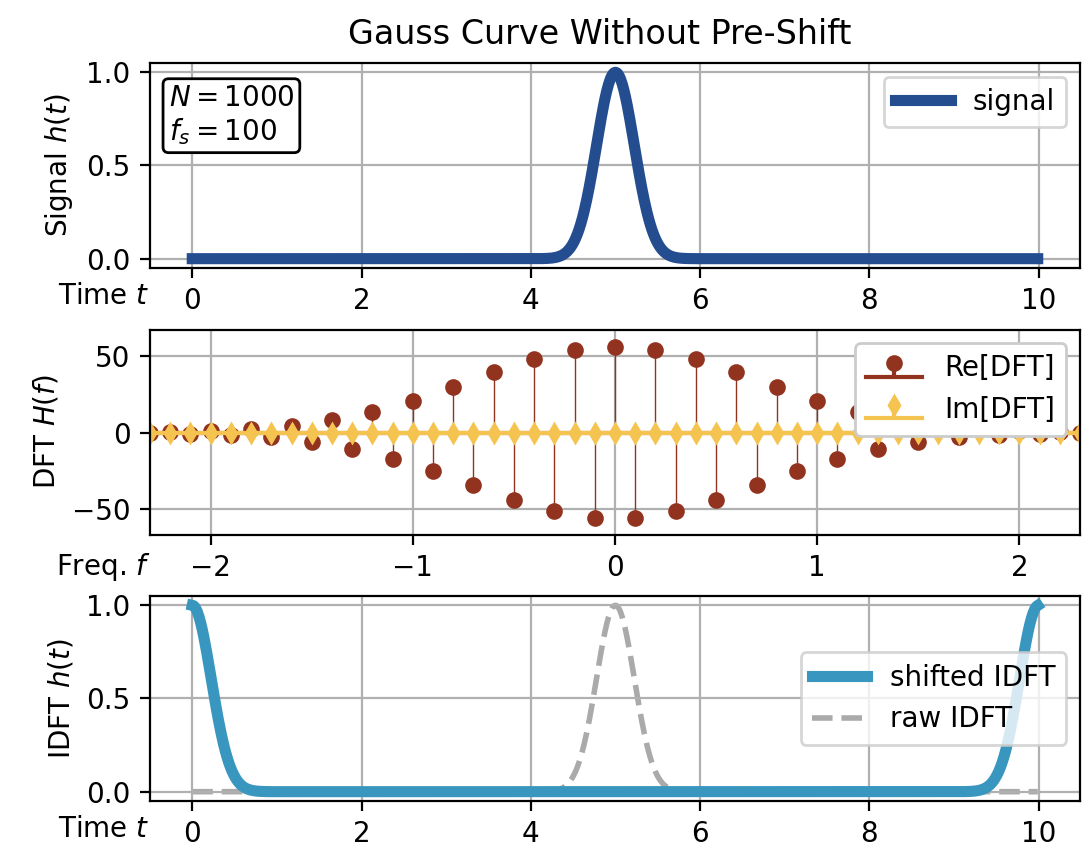
\includegraphics[width=\linewidth]{gauss-raw}
\caption{Directly computing the DFT of a Gauss curve. Since the input signal is shifted from the origin to $ t = 5 $, the DFT contains a corresponding modulation factor $ e^{-2\pi i k} $, which produces sinusoidal oscillation about the expected Gauss-curve envelope. The last graph shows the IDFT without \texttt{ifftshift} (in grey) and with \texttt{ifftshift} (blue).}
\label{dft:fig:gauss-raw}
\end{figure}

\begin{figure}
\centering
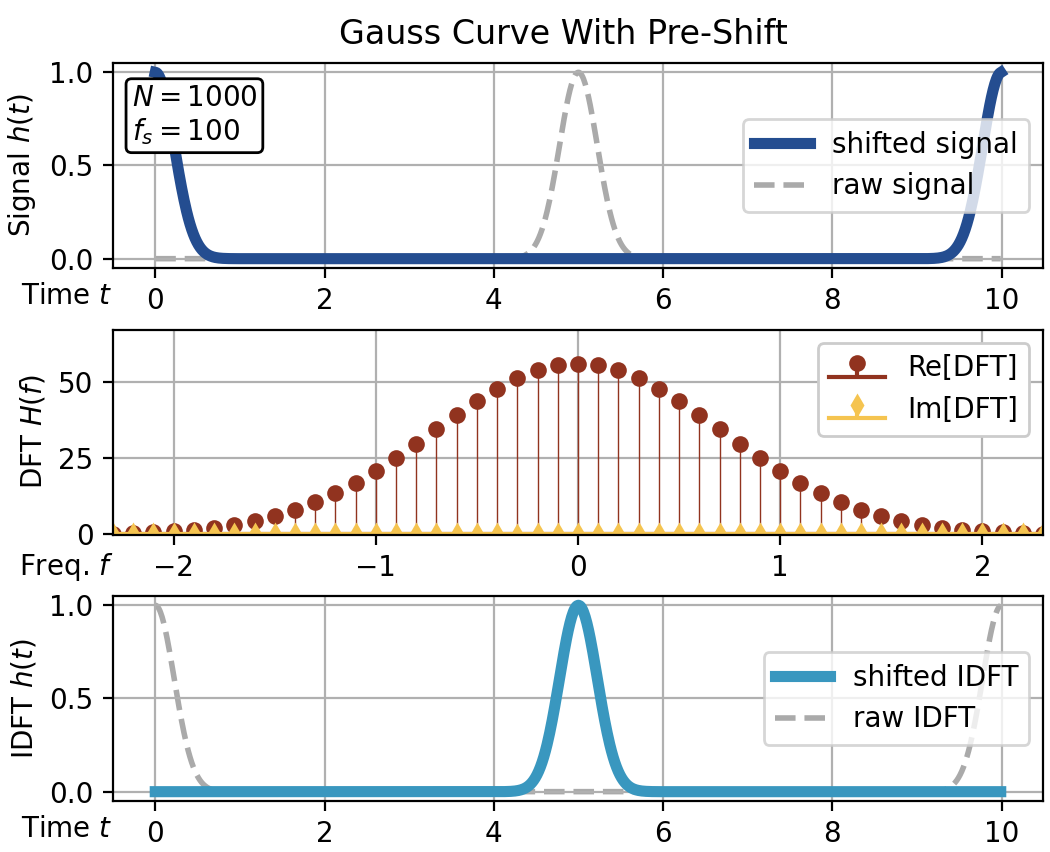
\includegraphics[width=\linewidth]{gauss-shifted}
\caption{DFT of a Gauss curve, take two. The input signal is made ``periodic'' by a pre-application of \texttt{fftshift}, which results in an unmodulated spectrum. The raw IDFT recovers the ``periodic'' input signal, while the shifted IDFT produces a raw, un-shifted Gauss curve.}
\label{dft:fig:gauss-shifted}
\end{figure}


\section{Sinusoids}
I used the simple combination of sinusoidal signals
\begin{equation}
	h(t) = \cos(2\pi f_{1} t) + 0.5 \cdot \sin(2\pi f_{2}t), \qquad f_{1} = 2, f_{2} = 5 \label{dft:eq:sinusoid}
\end{equation}
to investigate aliasing, spectral leakage, and zero padding. Figure \ref{dft:fig:sinusoids} shows the sinusoidal signal and its DFT without ``anything wrong,'' i.e. before I start tinkering when investigating aliasing, spectral leakage, etc... Note that the frequencies $ f_{1} = 2 $ and $ f_{2} = 5 $ are clearly visible in the spectrum, and that the frequency of the even harmonic---$ f_{1} = 2 $ from the cosine term---appears in the real portion of the DFT, while the odd sine frequency $ f_{2} = 5 $ appears in the imaginary portion of the DFT. Naturally, $ \Re(H(f_{k}) $ is an even function, while $ \Im(H(f_{k})  $ is odd. 


\begin{figure}[htb!]
\centering
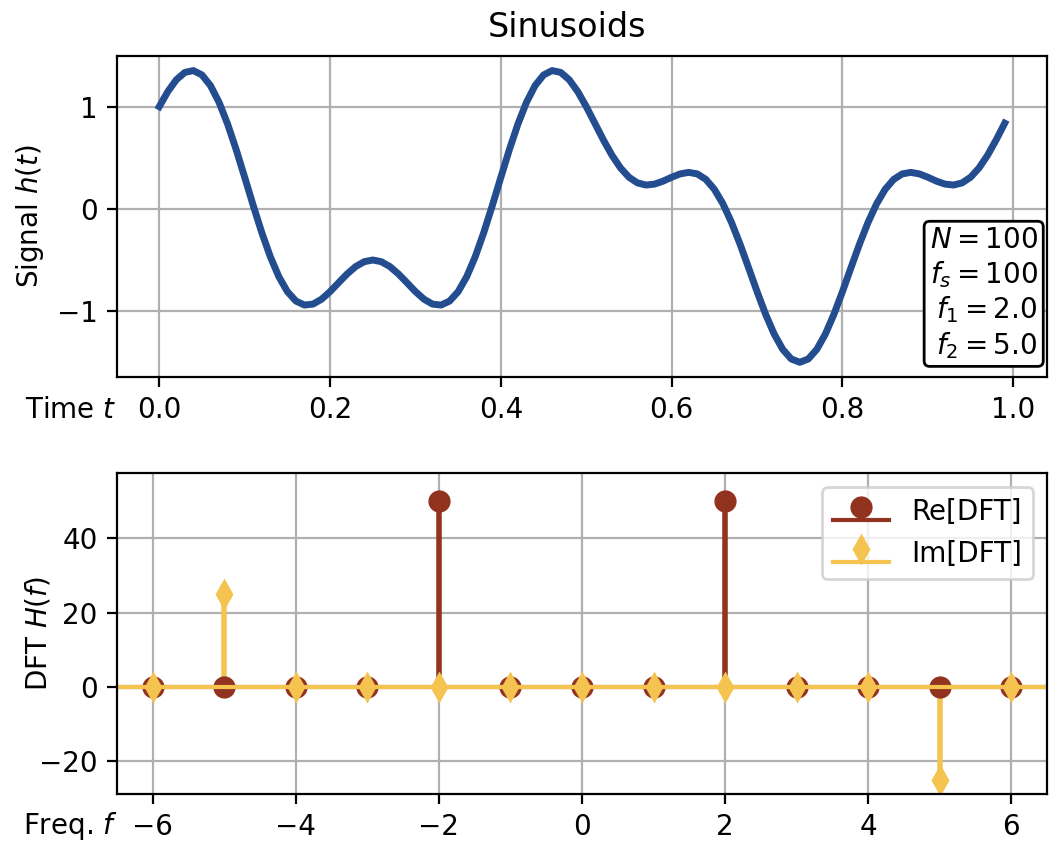
\includegraphics[width=\linewidth]{sinusoids}
\vspace{-6mm}
\caption{The unblemished waveform and spectrum of the sinusoidal signal (\ref{dft:eq:sinusoid}) used for the remainder of this section. Note the clearly visible frequencies $ f_{1} = 2 $ and $ f_{2} = 5 $.}
\label{dft:fig:sinusoids}
\end{figure}

\subsection{Aliasing}
To investigate aliasing---the DFT's distortion for input frequencies above the Nyquist limit---I lowered the frequency at which I sampled the signal (\ref{dft:eq:sinusoid}) until the Nyquist frequency $ f_{c} $ fell below the higher frequency $ f_{2} = 5 $. As expected, the DFT fails to properly detect the $ f_{2} $ frequency, which falls just outside the Nyquist limit and is instead mapped back into the spectrum's available bandwidth at an incorrect position. Unsurprisingly, the IDFT fails to reconstruct the original signal. The problematic effects of aliasing would be more prominent in a signal containing many frequencies above the Nyquist limit, as seen in the analysis of the Bach violin recording in  \hyperref[dft:s:bach]{Section \ref{dft:s:bach}}.


\begin{figure}[htb!]
\centering
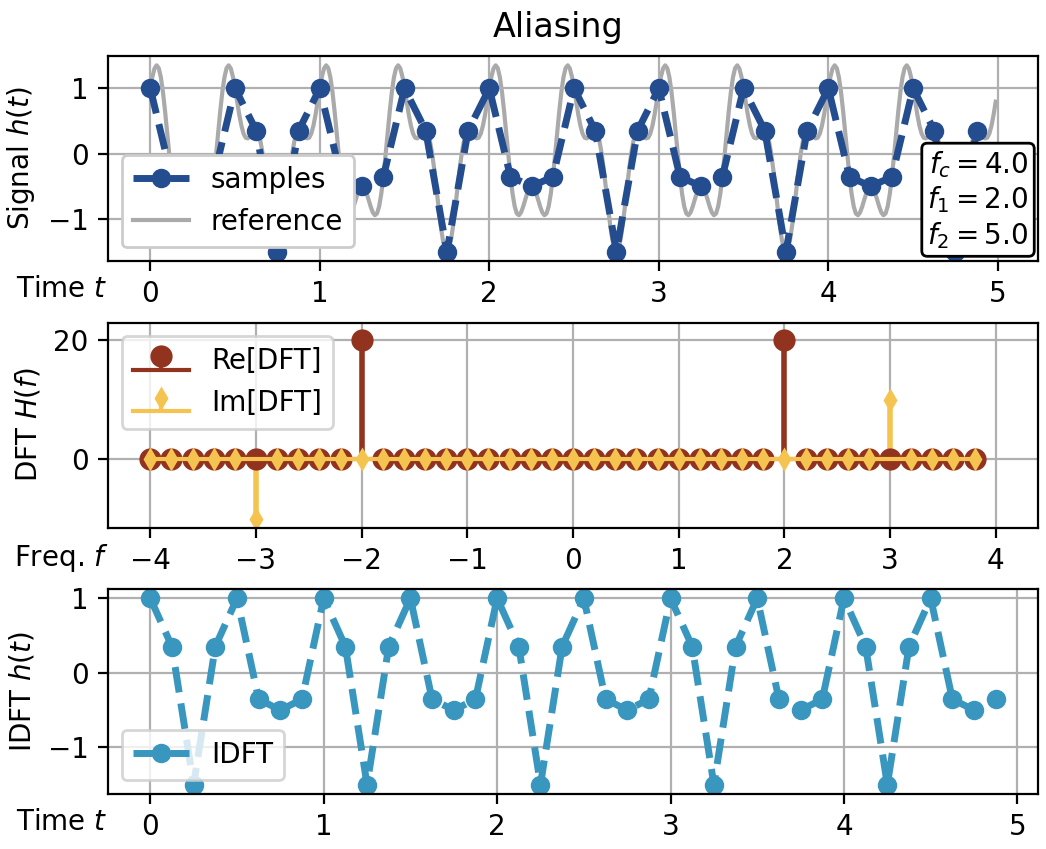
\includegraphics[width=\linewidth]{aliasing}
\vspace{-8mm}
\caption{The effects of aliasing when the Nyquist frequency is lowered below $ f_{2} = 5 $---the higher frequency $ f_{2} $ is mapped into the spectrum at an incorrect position, and the DFT and IDFT are accordingly distorted.}
\label{dft:fig:aliasing}
\end{figure}


\subsection{Spectral Leakage}
To investigate spectral leakage, I shifted the time over which I sampled the signal (\ref{dft:eq:sinusoid}) to roughly one-and-a-quarter periods. Resultantly,  the DFT's no long sees a periodic input, as visible in the top graph of Figure \ref{dft:fig:spectral-leakage}. The lack of periodicity wreaks havoc in the DFT, introducing a multitude of new frequencies and shifting existing ones from their correct positions. Unsurprisingly, the IDFT correspondingly fails to reproduce the original signal, which is shown for reference in the bottom graph.


\begin{figure}[htb!]
\centering
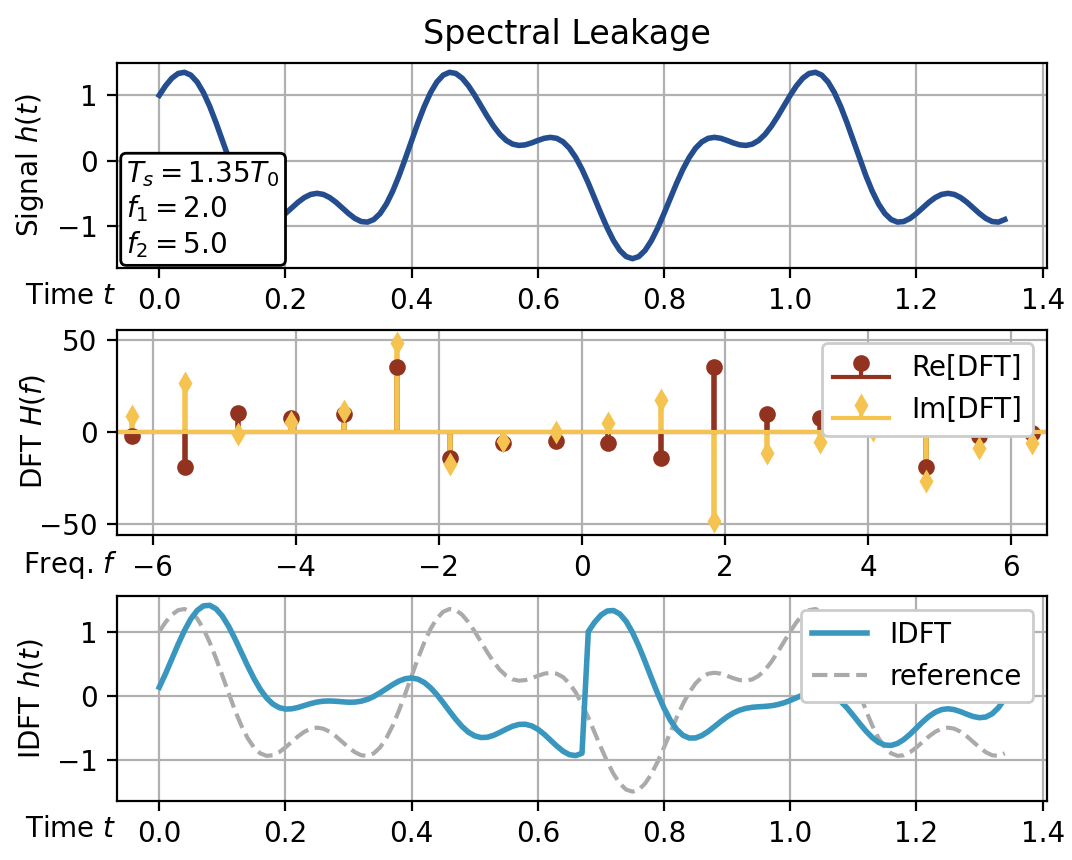
\includegraphics[width=\linewidth]{spectral-leakage}
\vspace{-8mm}
\caption{The effects of spectral leakage, which occurs when the input signal is not periodic over the sampling time. Spectral leakage introduces new frequencies, shifts the existing frequencies from their true values, and produces an incorrect inverse transform (the correct version is shown in dashed gray for reference).}
\label{dft:fig:spectral-leakage}
\end{figure}


\subsection{Zero Padding}
To investigate the use of zero padding, I decreased the time over which I sampled the signal (\ref{dft:eq:sinusoid}) to slightly less than one period, as shown in the top graph of Figure \ref{dft:fig:zero-padding}. Accordingly, the DFT suffers from poor spectral resolution and fails to accurately identify the two frequencies $ f_{1} = 2 $ and $ f_{2} = 5 $. This is remedied by zero padding---appending a large number of zeros to the input signal with the hope of artificially increasing resolution with increased sample duration. In my case, I appending zeros amounting to 10 times the number of original samples (not shown in the graph because the signal grows too compressed to be recognizable). 

In practice, zero padding works as a sort of interpolation that connects the points of a sparsely populated spectrum. It doesn't add more information to an existing spectrum, but helps reveal, via the extrema positions of the zero padded DFT, information that is already present, just not easily visible. Figure \ref{dft:fig:zero-padding} shows the results---indeed, the zero padded DFT helps identify the $ f_{1} = 2 $ and $ f_{2} = 5 $, which hidden in the raw spectrum.

I was pleasantly surprised to see that, although the inverse transform of the non-padded DFT fails to correctly reproduce the original signal, the inverse transform of the zero padded DFT does so almost flawlessly.  

\begin{figure}[htb!]
\centering
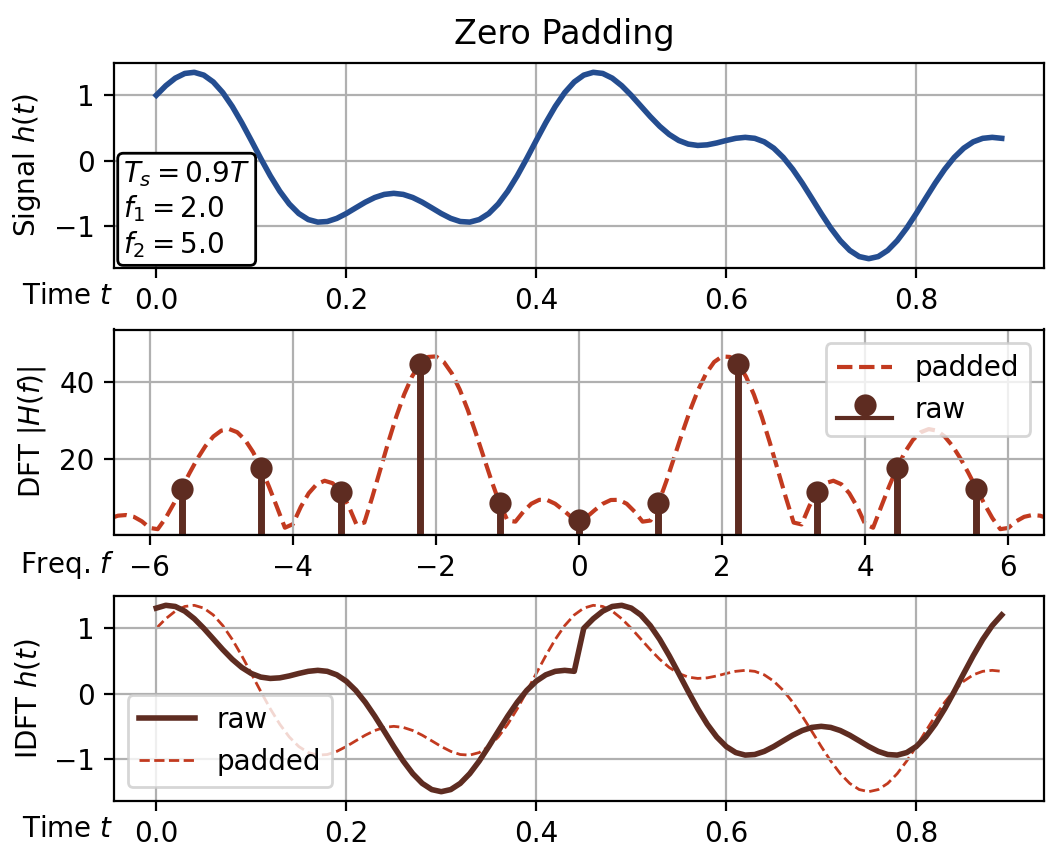
\includegraphics[width=\linewidth]{zero-padding}
\vspace{-8mm}
\caption{The use of zero padding to identify spectrum frequencies. The raw signal is increased in length by a factor of ten by appending zeros to the end (not shown), and the zero padded DFT's extrema positions reveal the frequencies the $ f_{1} = 2 $ and $ f_{2} = 5 $. Note that zero padding also improves the accuracy of the inverse DFT.}
\label{dft:fig:zero-padding}
\end{figure}



\section{Computation Times} \label{dft:s:times}
I compared the computation times of four DFT implementations: the loop and matrix algorithms in  \hyperref[dft:ss:dft-algorithms]{Section \ref{dft:ss:dft-algorithms}}, Numpy's \texttt{fft}, which uses the fast Fourier transform, and Numpy's \texttt{fftr}, which is a fast Fourier transform optimized for real input. I measured the time each method took to compute the discrete Fourier transform of the sinusoidal signal $ h(t) = \sin(2\pi \cdot 10 \cdot t) $ sampled at $ N $ points on the interval $ [0, 10] $. Figure \ref{dft:fig:times} shows the results.

Unsurprisingly, both FFT methods superlatively outperform my ``handmade'' implementations. Although the optimized \texttt{fftr} slightly outperforms \texttt{fft}, the difference is minimal for the small $ N $ I tested and is visible only on a logarithmic scale. Of my two basic DFT implementations, the matrix approach performs considerably better, likely by avoiding the explicit use of an expensive nested loop. In any case, both handmade methods show prohibitive asymptotic growth for consideration in any serious practical application. As a side note, since the matrix approach loads an entire $ N \cross N $ matrix into memory at once, it likely becomes prohibitively memory intensive for very large $ N $. That said, I didn't have any problems on my  $\SI{8}{GB}$ RAM computer for the moderate $ N $ I tested.

\begin{figure}
\centering
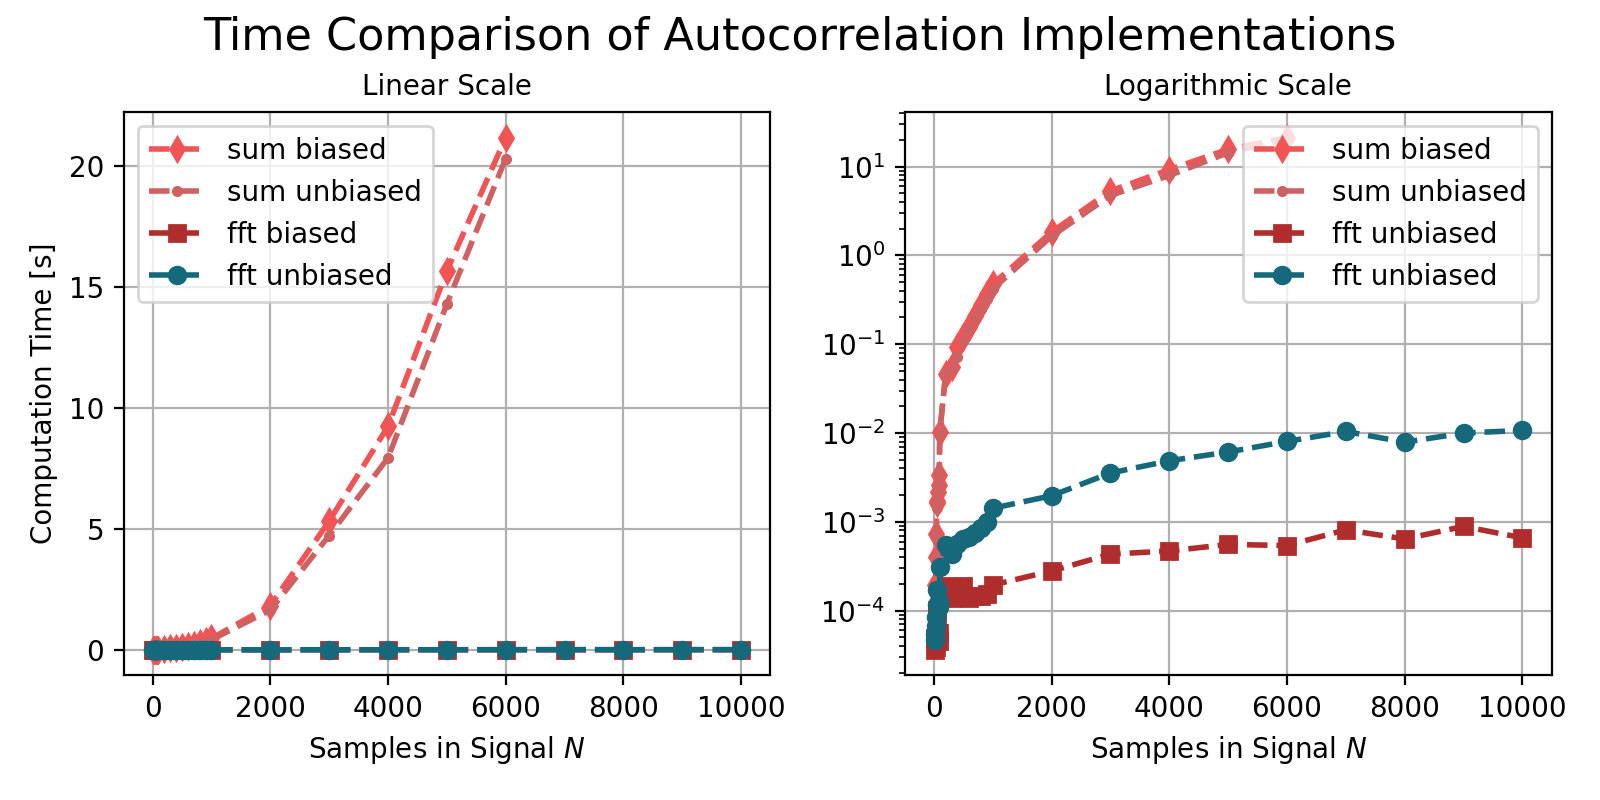
\includegraphics[width=\linewidth]{times}
\vspace{-7mm}
\caption{Time required for each of the four DFT implementations to compute the discrete Fourier transform of an $ N $-sample signal. Note the vast superiority of the FFT implementations.}
\label{dft:fig:times}
\end{figure}


\section{Analyzing a Bach Partita} \label{dft:s:bach}
First, some background: we are given a short excerpt from a Bach violin partita, recorded at the sample rates 44100, 11025, 5512, 2756, 1378,  and \SI{882}{\hertz}. As the sample rate decreases, I notice two main trends:
\begin{enumerate}
	\item The recording sounds increasingly distorted
	\item Higher frequencies disappear from the recording, and accordingly, the violin's distinctive timbre vanishes with the higher harmonics
\end{enumerate}
My first step was to try to find the musical notes played in the recording, which would tell me the corresponding frequencies and thus provide a quantitative reference for my analysis. Since I don't have perfect pitch, I turned to YouTube for improvised research. As far as I can tell, the sample recording comes from the opening seconds of the fourth movement, \textit{Double (Presto)}, of Bach's Partita No. 1 in B minor, BWV 1002. Figure \ref{dft:fig:sheet-music} shows the corresponding sheet music.

\begin{figure}[htb!]
\centering
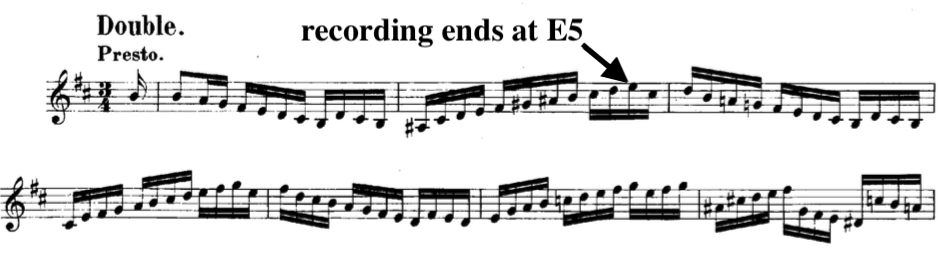
\includegraphics[width=\linewidth]{sheet-music-annotated}
\caption{The partita's first few measures. Our sample recording ends at the \texttt{E5} note in the third measure.}
\label{dft:fig:sheet-music}
\end{figure}

In order, the notes in the excerpt are
\begin{quote}
	\texttt{B4 B4 A4 G4 F\#4 E4 D4 C\#4 B3 D4 C\#4 B3}\\ \texttt{A\#3 C\#4 D4 E4 D4 G\#4 A\#4 B4 C\#5 D5 E5}
\end{quote}
The notes span the frequency range from a low \SI{233.1}{\hertz} at \texttt{A\#3} to a high \SI{659.3}{\hertz} at \texttt{E5}. Figure \ref{dft:fig:first-note} shows the spectrum of the opening note, a \texttt{B4} with frequency \SI{493.9}{\hertz}, for each sample rate. Clearly, decreasing the sample rate, and thus the Nyquist frequency, removes higher harmonics and leads to aliasing, progressively degrading the recording's fidelity. At \SI{5512}{\hertz} and below, the opening note is no longer recognizable as a \texttt{B4}, discussed more below. Figure \ref{dft:fig:partita-spectrum} shows the analogous spectra of the entire recording and displays similar problems with aliasing and higher harmonics.

\begin{figure}[htb!]
\centering
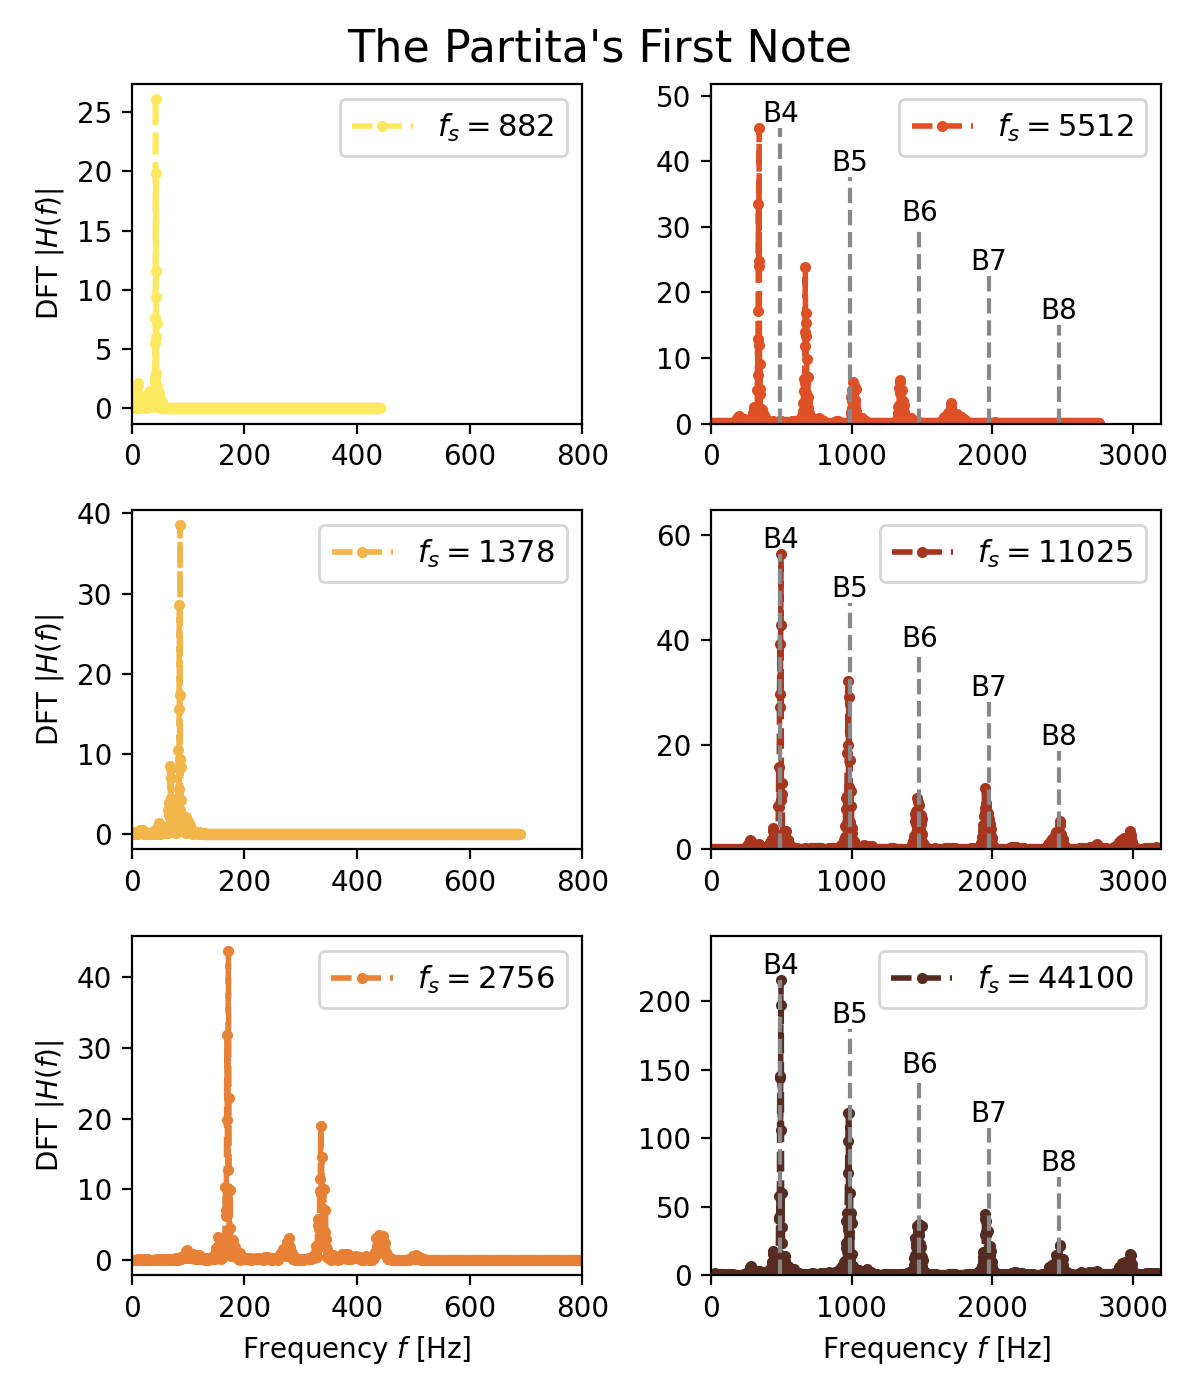
\includegraphics[width=\linewidth]{partita-first-note}
\vspace{-8mm}
\caption{Spectrum of the partita's first note, a \SI{493}{\hertz} \texttt{B4}. For the highest three sample rates, the theoretically expected positions of the note and its higher harmonics are shown for reference. Note the agreement at 44100 and \SI{11025}{\hertz} and disagreement at (and below; not shown) \SI{5512}{\hertz}, meaning the note is no longer recognizable as a \texttt{B}. In general, the spectrum grows weaker and more aliased with decreasing sample rate.}
\label{dft:fig:first-note}
\end{figure}



An analysis of the change in sound quality with sample rate follows, with attempts at an explanation using the lessons of Fourier analysis. 
\begin{itemize}
	\item At \SI{44100}{\hertz} the recording sounds excellent, at least to my non-expert ears. The instrument is clearly a violin. In the spectra of both the first note and the entire recording, higher harmonics are clearly visible.
	
	\item At \SI{11025}{\hertz}, the recording sounds a bit ``hollow''---it appears that the high harmonics (which are quite weak) are cut off and aliased into the available spectral bandwidth below the Nyquist frequency $ f_{c} = \SI{5512}{\hertz} $. Nonetheless, the effect is minimal and, if I am honest, I am not sure I would detect something is wrong with the recording without \textit{a priori} knowledge. This stance is validated by comparing the spectra of the \SI{44100}{\hertz} and \SI{11025}{\hertz} samples---they are nearly identical, at least up to the \SI{11025}{\hertz} recording's Nyquist frequency.
	
	\item By \SI{5512}{\hertz}, the recording is audibly distorted, and the distinctive violin sound is fading. A look at the spectra suggest the lack of harmonics beyond $  f_{c}  \approx \SI{2750}{\hertz} $ and a general shift to lower frequencies is to blame. In particular, the spectrum of the first note at \SI{5512}{\hertz} shows periodic frequencies, but these are no longer integer multiples of the fundamental frequency, and fail to match the actual \texttt{B4} note or its higher harmonics from the original sheet music.
	
	\item At \SI{2756}{\hertz}, I can hardly recognize the instrument is a violin, since the instrument's timbre---a fancy word for the instrument's distinctive sound or musical ``fingerprint''---is progressively erased along with the higher harmonics, as confirmed in the spectra as the Nyquist frequency decreases.
	
	\item By \SI{1378}{\hertz}, I can just barely make out the melody. This agrees with theory---although the sample rate is very low, even the highest fundamental frequency in the melody, the \texttt{E5}'s \SI{569}{\hertz}, still falls withing the \SI{689}{\hertz} Nyquist range, so it makes sense that the melody is still (barely) distinguishable.
	
	\item At \SI{882}{\hertz} sampling, I can no longer detect the melody, since even the melody's fundamental frequencies begin to exceed the \SI{441}{\hertz} Nyquist limit. The recording is devoid of high frequencies and is strongly distorted, corresponding to a spectrum muddled by aliasing and stripped of frequencies above \SI{440}{\hertz}. 
	
\end{itemize} 



\begin{figure}[htb!]
\centering
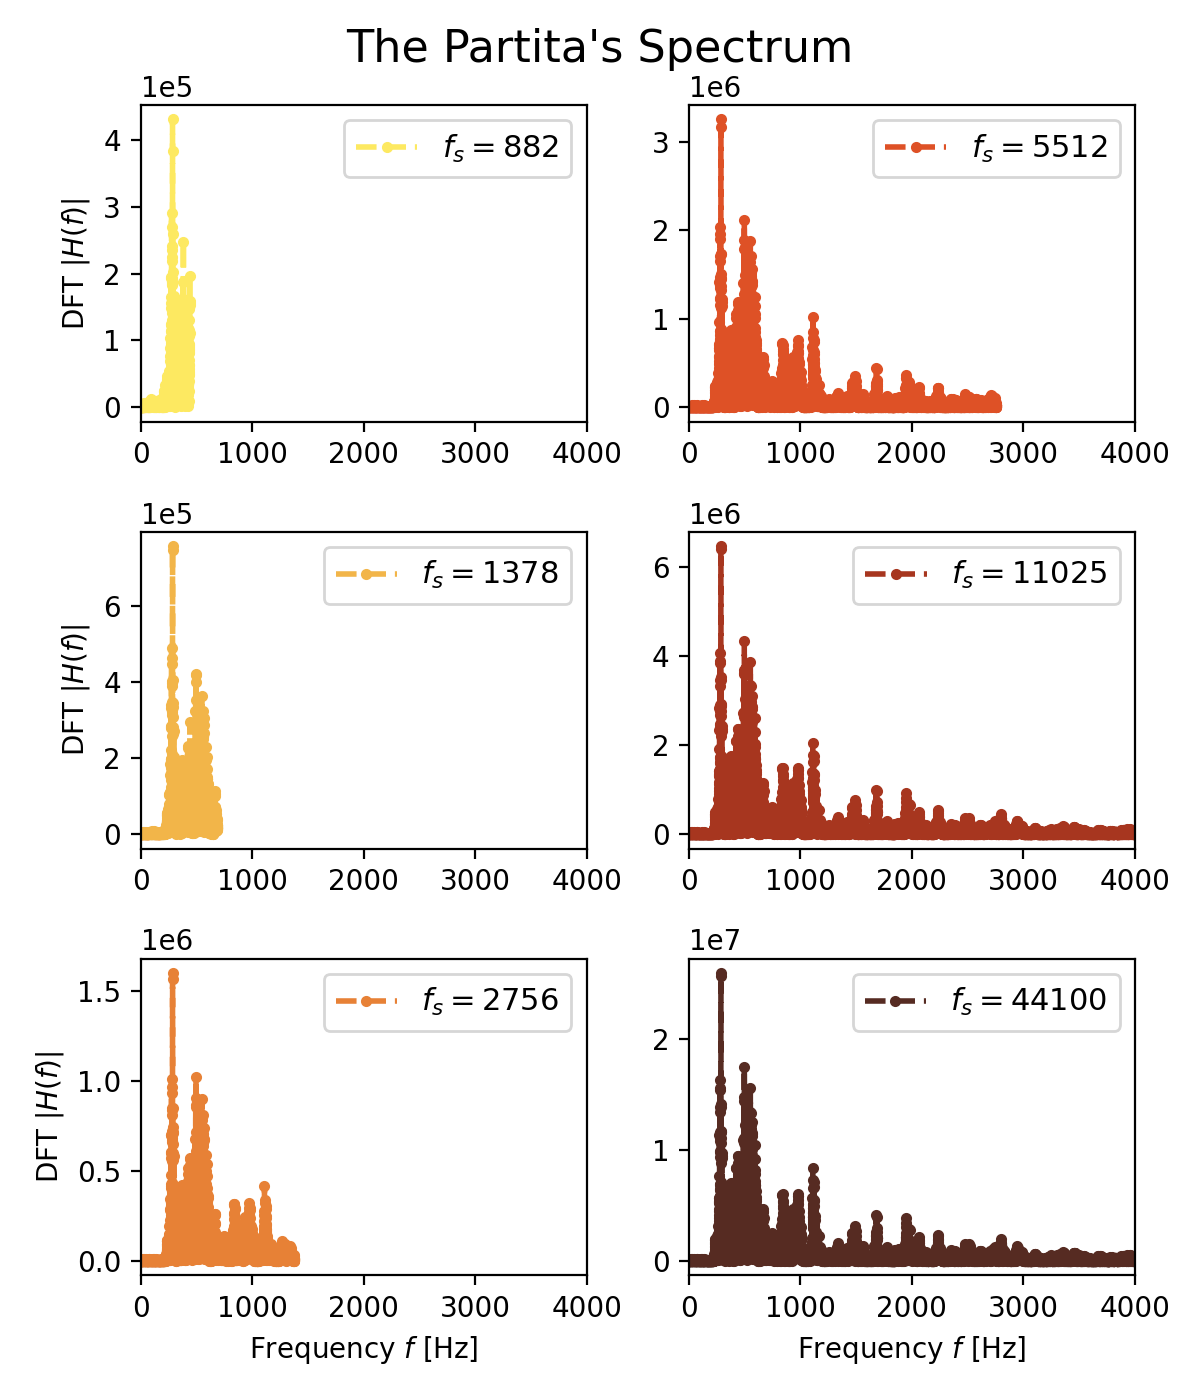
\includegraphics[width=\linewidth]{partita-spectrum}
\vspace{-8mm}
\caption{The entire recording's spectrum at various sample rates. Note that the 44100 and \SI{11025}{\hertz} spectra are nearly identical (at least below the Nyquist limit, beyond the graph's axis limits). Besides the obvious truncation of harmonics and aliasing at lower sample rates, note that spectrum's amplitude grows weaker as well.}
\label{dft:fig:partita-spectrum}
\end{figure}


\section{Extra: Decomposing Guitar Chords}

\subsection{Extracting Notes in the Chords}
For this section, I recorded a few simple chords on a nylon-string acoustic guitar in \texttt{wav} format at \SI{44100}{\hertz}, and then attempted to extract the chords' constituent notes using the DFT. Since I knew the notes in each chord \textit{a priori} (e.g. an A major chord played across all six string contains the notes \texttt{A2}, \texttt{E3}, \texttt{A3}, \texttt{C\#4}, \texttt{E4} and \texttt{A4}), I could assign each note a corresponding frequency using the 12-tone equal temperament tuning system. 

To avoid bogging down this report with music theory, I'll refer interested readers to \cite{twelve-tet}. For our purposes, it is enough to know that we can bijectively map each note to a corresponding frequency (see e.g. \cite{note-freqs} for tabulated values). I could then theoretically predict which frequencies ``should'' be present in a given chord. My goal was to test if the theoretically expected frequencies agreed with the experimental data from a DFT analysis of the \texttt{wav} files. 

Happily, the experiment worked! Figure \ref{dft:fig:chords} shows the results. The dashed gray lines show the theoretically expected positions of the chords' notes and their first few harmonics, in good agreement with the spectral peaks.


\begin{figure}[htb!]
\centering
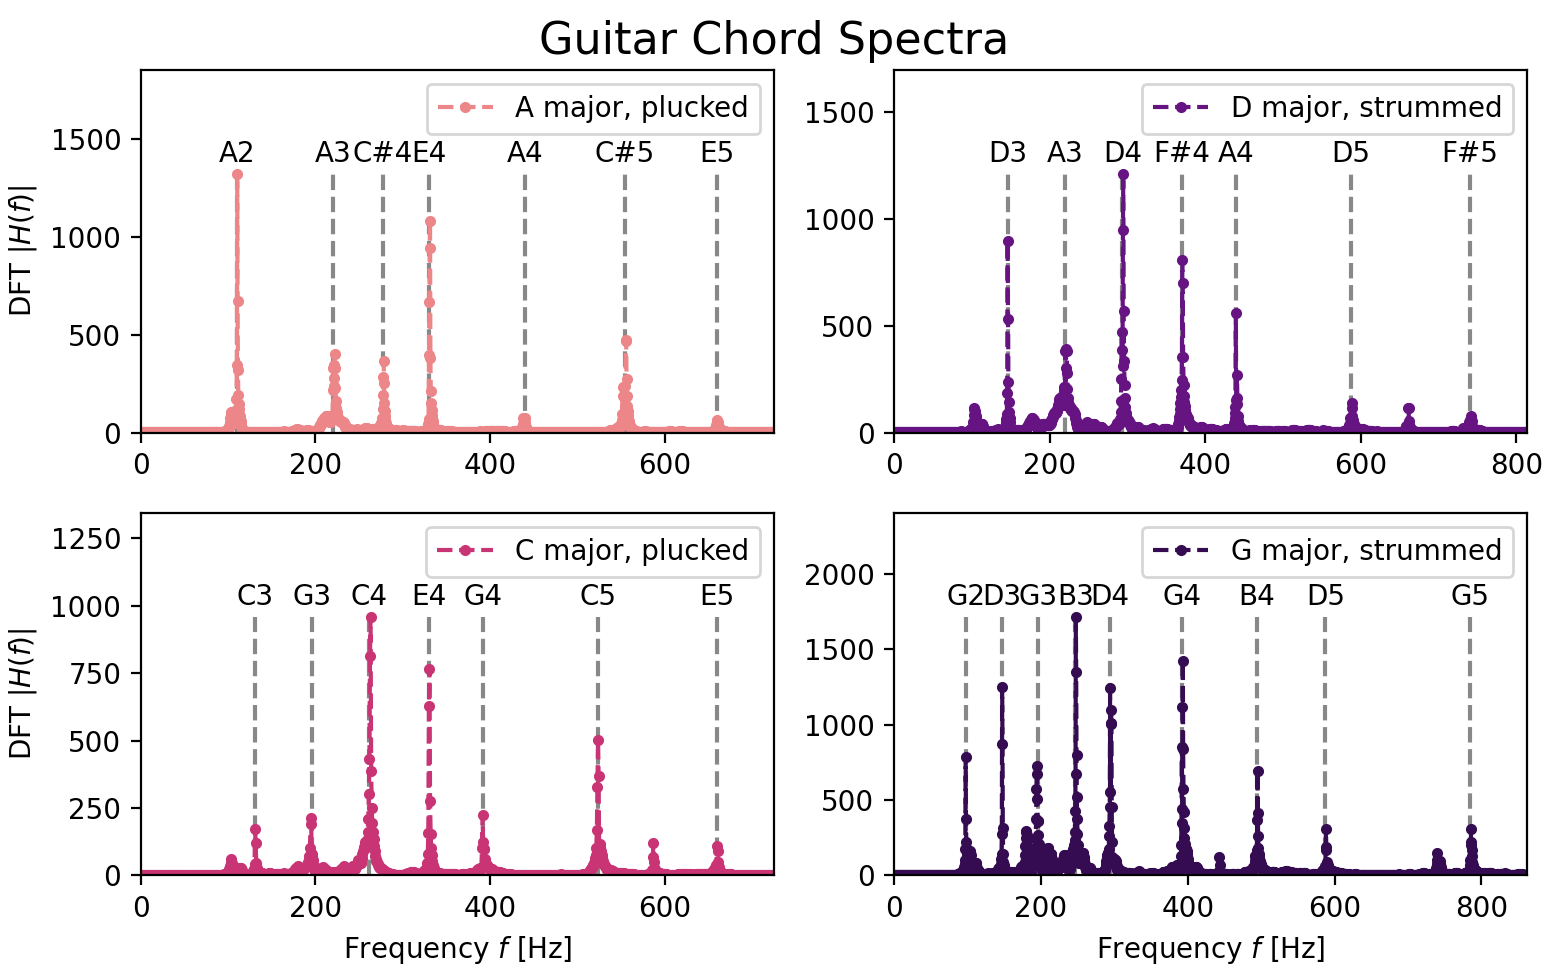
\includegraphics[width=\linewidth]{chords}
\vspace{-8mm}
\caption{Comparing the theoretically expected notes (dashed grey lines and labels) in nylon-string acoustic guitar chords to the chords' spectra. Note the good agreement in all four cases. The frequency positions are found using the 12-tone equal temperament tuning system described in \cite{twelve-tet}.}
\label{dft:fig:chords}
\end{figure}



\subsection{Detecting Slightly Flat Tuning}
As a last experiment, I intentionally tuned my guitar \SI{8}{\hertz} flat relative to the standard \texttt{A4} frequency of \SI{440}{\hertz}, ending up with a reference tone of \texttt{A4} $\mapsto$ \SI{432}{\hertz}. I recorded (again in \texttt{wav} format at \SI{44100}{\hertz}) a few simple chords in \SI{432}{\hertz} tuning and compared them to a \SI{440}{\hertz} reference version. I was curious to see if the DFT would detect the slight difference in the tuning. Figure \ref{dft:fig:chord-440-432} shows the results for a strummed A major chord, with the \SI{440}{\hertz} and \SI{432}{\hertz} versions plotted on the same axis, along with the theoretically expected constituent note positions for each tuning system. The difference is subtle, but present---the \SI{432}{\hertz} chord is shifted to slightly lower frequencies.


\begin{figure}[htb!]
\centering
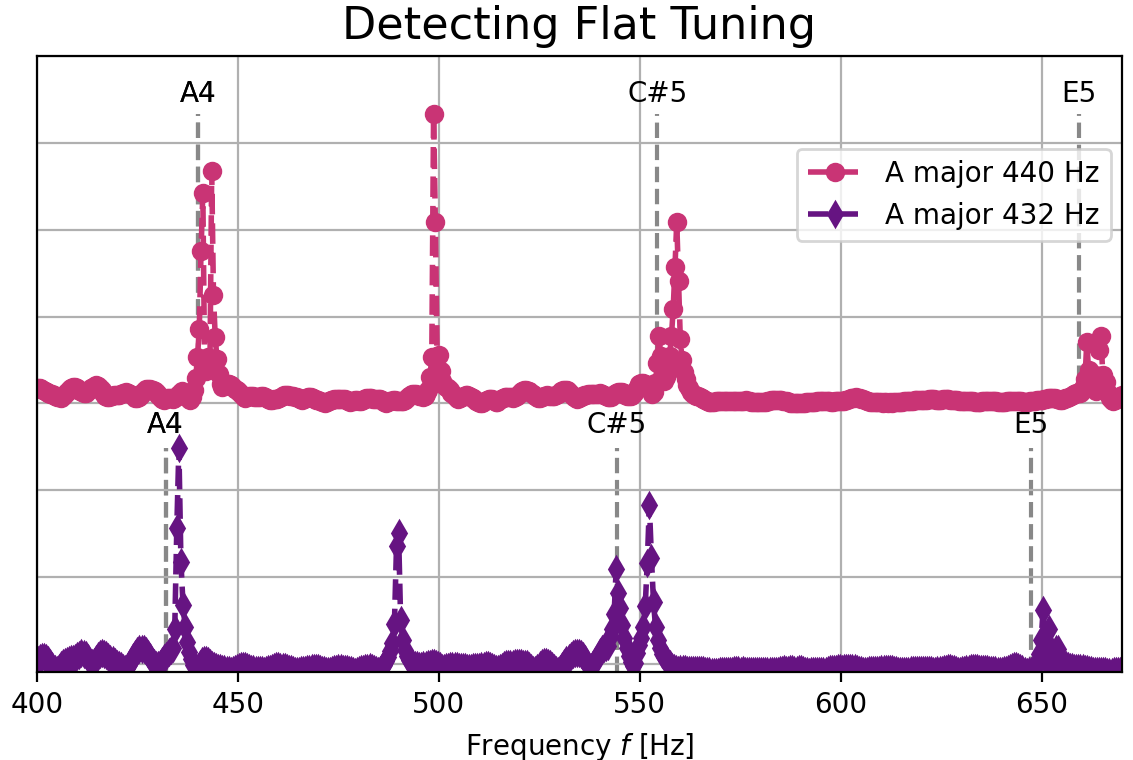
\includegraphics[width=\linewidth]{chord-440-432}
\vspace{-8mm}
\caption{Comparing an A major chord in \SI{440}{\hertz} and \SI{432}{\hertz} tuning. As expected, the \SI{432}{\hertz} version's notes and spectral peaks are shifted to slightly lower frequencies.}
\label{dft:fig:chord-440-432}
\end{figure}
 



\begin{thebibliography}{}
\setlength{\itemsep}{.2\itemsep}\setlength{\parsep}{.5\parsep}

\bibitem{dsp-online} ``Spectral Leakage and Zero Padding of the Discrete Fourier Transform''. \url{https://dspillustrations.com/pages/posts/misc/spectral-leakage-zero padding-and-frequency-resolution.html}

\bibitem{wiki-shift} Wikipedia contributors. "Discrete Fourier transform." \textit{Wikipedia, The Free Encyclopedia}. 1 November 2020. \url{https://en.wikipedia.org/wiki/Discrete_Fourier_transform#Shift_theorem}


\bibitem{note-freqs} B. H. Suits. ``Frequencies for equal-tempered scale, A4 = 440 Hz'' Physics Department, Michigan Technological University. \url{https://pages.mtu.edu/~suits/notefreqs.html}

\bibitem{twelve-tet} Wikipedia contributors. "12 equal temperament." \textit{Wikipedia, The Free Encyclopedia}. 27 October 2020. \url{https://en.wikipedia.org/wiki/12_equal_temperament#Mathematical_properties}.


\end{thebibliography}

\end{document}



%Sheet music source: https://imslp.org/wiki/Violin_Partita_No.1_in_B_minor%2C_BWV_1002_(Bach%2C_Johann_Sebastian)
